\documentclass[11pt]{article}

\usepackage{graphicx}

\usepackage[left=2cm, right=2cm, top=2cm, bottom=2cm]{geometry}

\title{SmartCity used by Paris, London, New York and Tokyo!}
\author{Guillaume Cluzel, Vincent Rébiscoul}
\date{21 Décembre 2018}

\begin{document}
\maketitle

\section*{Introduction}

Créer une smart city requiert d'utiliser un grand nombre de capteurs à travers toute la ville. Pour améliorer le fonctionnement de la ville, il est nécessaire de modéliser ces capteurs pour tirer des valeurs et faire des modélisations. La modélisation de ces capteurs nécessite de créer un méta modèle représentant cet ensemble de capteurs. Nous le présenterons dans un premier temps, ainsi que ses différentes capacités.

Pour utiliser facilement ce méta modèle et pour modéliser facilement nos capteurs, nous utilisons un DSL graphique. Nous expliquons ce choix et présentons notre DSL dans une seconde partie.

Dans une troisième partie nous montrerons comment nous avons implémenté une extension de notre DSL, et la raison pour laquelle nous l'avons considérée.

Enfin nous verrons d'une manière critique ce qui pourrait être amélioré.

Une dernière partie nous permettra de réfléchir à l'utilité d'un DSL pour modéliser notre ville.

\bigskip

Notre projet utilise le langage Java qui nous semblait être l'un des plus approprié, puisque c'est un langage orienté objet donc particulièrement adapté à la réalisation de méta modèles. Il possède une importe bibliothèque standard et donc de vastes possibilités en terme d'interface graphique, et une bonne aide sur internet ce qui a été utile pour les débutants que nous sommes. Nous avons néanmoins trouvé intéressant d'explorer une autre branche des DSL (les DSL graphiques) dans ce projet.

Dans tout notre travail, la base de données que nous avons utilisée s'appelle \textit{sec}.



\section{Meta-model}

Notre smart city est composé de plusieurs capteurs regroupé dans la classe \texttt{Sensor}. Plus généralement la partie jaune représente ce qui est lié à chaque sensor, c'est un dire le capteur en lui-même ainsi qu'un repérage spatial qui peut être utile pour repérer précisément chaque capteur dans la ville.

La partie bleue représente elle tout ce qui est données, c'est-à-dire les données en elles-mêmes captés par les capteurs sous le nom de \texttt{Mesurements} regroupé en \texttt{Data}. Il est également possible d'ouvrir des fichiers CSV et JSON facilement. 
Toutes les mesures faites peuvent ensuite être déformées par un \texttt{TailorMesurement} qui peut être soit un bruit ou un offset ajouté à chaque valeur du \texttt{Data}.

Enfin une partie blanche permet d'acquérir des données en les simulant. Différentes lois ont été implémentées, certaines basiques, d'autres plus complexes. On trouve:
\begin{itemize}
\item \texttt{RandomValues} : valeurs aléatoires entières
\item \texttt{RandomValuesFromSet} : valeur aléatoire prise dans un ensemble données \texttt{values}.
\item \texttt{MarkovChain} : représente des chaînes de Markov
\item \texttt{Function} : représentes des fonctions du temps qui retourne des valeurs Double.
\item \texttt{Interpolation} : Interpolation de plusieurs points pour donner des fonctions linéaires par morceaux.
\end{itemize}



Enfin pour générer nos données, on utilise la classe \texttt{GenerateData} qui permet de générer des données en temps réel, ou bien de générer des données qui pourront être envoyées par la suite toute en même temps.


\begin{figure}
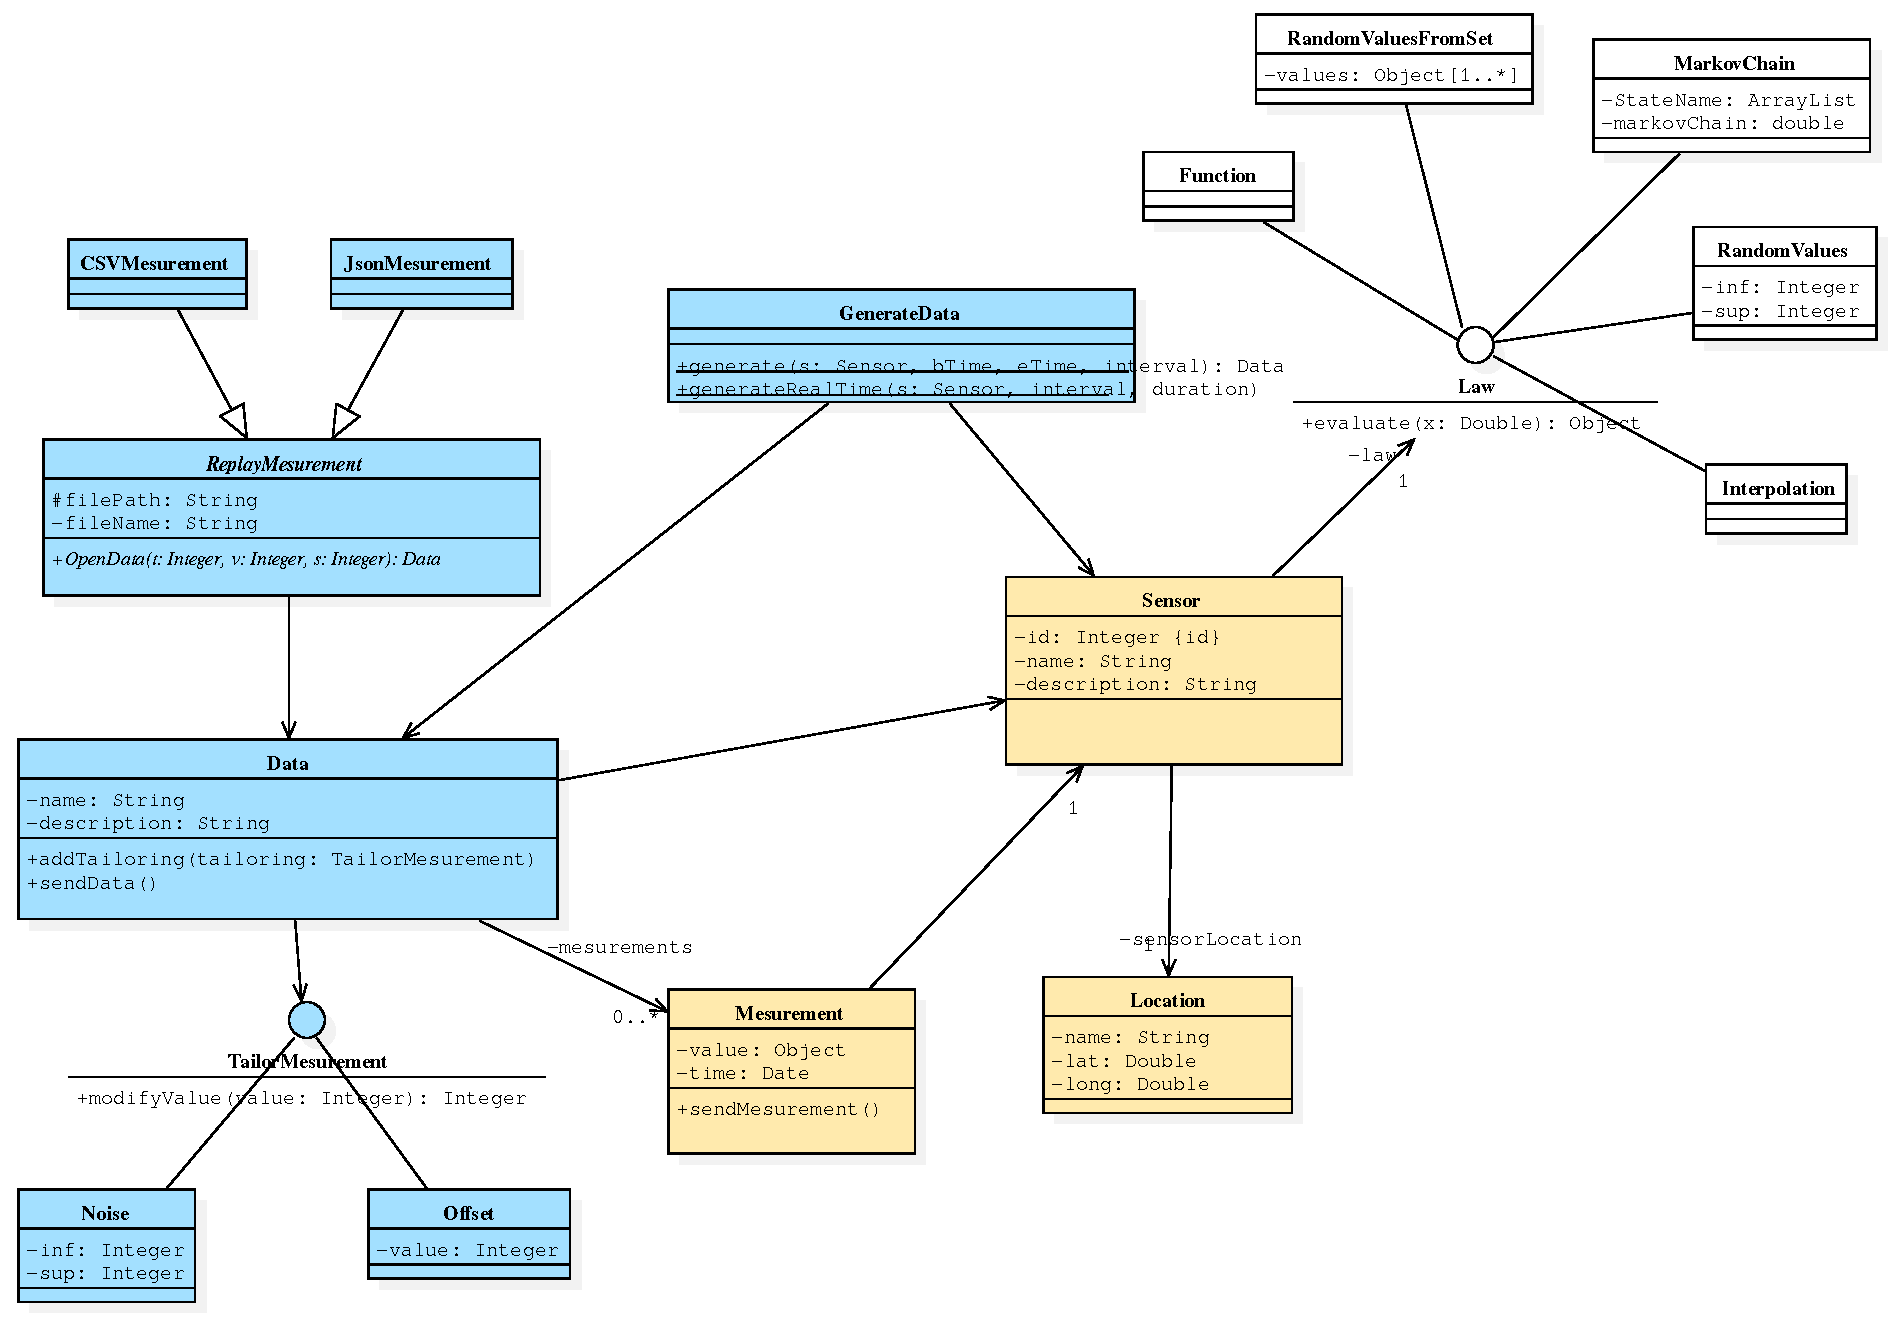
\includegraphics[width=\textwidth]{Figs/Main.pdf}
\caption{Meta modèle de notre smart city}
\end{figure}




\section{DSL graphique}

Pour ce projet, nous avons décidé de réaliser un DSL graphique. En effet, il semble raisonnable de penser que certains utilisateurs potentiels ne soient pas familiers avec la programmation. Or un DSL graphique semble être une bonne manière de créer un cadre de simulation d'une SmartCity (ou d'un SmartCampus) de manière accessible à un large public en restant le plus expressif possible. Notre interface permet de facilement créer des sensors, de leurs associer une loi, et de simuler le sensor sur une période de temps que l'utilisateur peut préciser. Il est également possible de modifier les données pour leur ajouter un offset ou un bruit facilement. L'envoie se fait à l'aide d'un simple bouton. L'envoie en temps réel lui aussi est implémenté via un bouton.

Plusieurs captures d'écran montrent les différents écrans de notre DSL et les différentes fenêtres permettant de réaliser toutes les actions souhaitées, avec dans l'ordre la création d'un nouveau sensor, la fênetre permettant de lancer une nouvelle simulation pour un sensor, la fenêtre qui permet de créer une nouvelle variation dans les données. Ces fênetres sont montrées à la figure \ref{fig:fen};

\begin{figure}
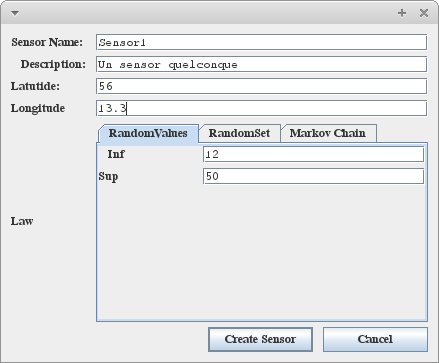
\includegraphics[scale=.4]{Figs/nsensor.png}
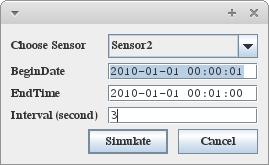
\includegraphics[scale=.5]{Figs/simul}
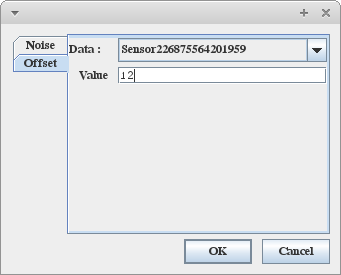
\includegraphics[scale=.5]{Figs/tailoring}
\caption{Différentes fenêtres de notre DSL}
 \label{fig:fen}
\end{figure}

Enfin on a une vue générale de notre interface graphique sur la figure \ref{fig:intro}.

\begin{figure}
  \centering
  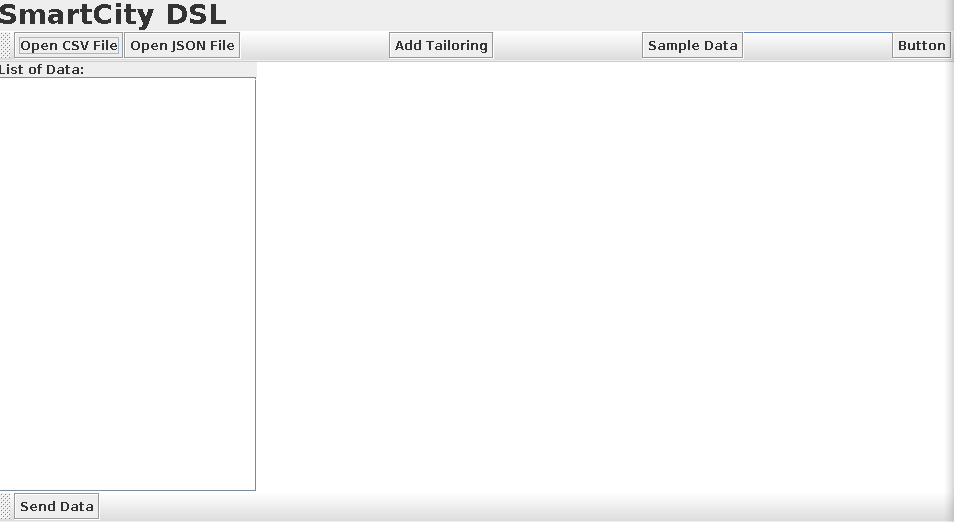
\includegraphics[width=\textwidth]{Figs/intro.png}
  \caption{The main window of our graphical DSL}
  \label{fig:intro}
\end{figure}


Pour aider l'utilisateur quand des entrées on un format nécessaire à respecter, nous avons entré directement le format à respecter. C'est notamment le cas pour les dates.

Pour faciliter les saisies, notamment pour les chaînes de markov qui pourraient être fastidieuses à entrer à la main à chaque utilisation, nous utilisons un fichier CSV pour les enregistrer et nous ouvrons simplement le fichier CSV.

Bien sûr, aucun de nous deux n'est expert en Java, et encore moins en interface graphique. Elle possède donc de sérieuses limitations, premièrement par le fait que nous ne sommes pas familier avec tous les composants et que nous n'utilisons pas forcément les plus adaptés. Nous ne sommes pas non plus des experts en interface graphique ce qui s'en ressent sur l'ergonomie.



\section{Notre extension}


Nous avons choisi l'extension ``E4: Real Time Simulations''. Nous avons en effet choisi cette extension car modéliser en temps réel un system a un intérêt pour voir s'il est robuste sur la durée.

Une modélisation en temps réel ressemble à une modélisation normale. Sauf que chaque valeur est générée à intervalle constant et directement envoyée dans la base de données.

Nous avons essayer de créer notre extension de manière à avoir le moins possible de code à réécrire par rapport à une simulation standard.

Un simple Thread.sleep permet de faire une pause et passer à la valeur suivante. La seule limitation est qu'il devient impossible de faire autre chose en même temps que l'envoie des données se passe. Il pourrait être intéressant de modifier cela pour que l'envoie des données devienne une tâche d'arrière plan dans un nouveau Thread.


\section{Critique de notre projet}

Un désaventage majeur de notre projet et qu'on n'a implémenté aucune fonction pour exporter des données). Il aurait fallu dans l'idéal créer des fonctions permettant d'exporter
\begin{itemize}
\item Des données qui ont été généré directement dans notre logiciel pour pouvoir les réutiliser plus tard dans notre logiciel directement.
\item L'environnement de travail, c'est-à-dire l'ensemble de nos sensors et les lois qui leur sont associées. En effet il est assez pénible à chaque nouvelle ouverture de fichier de devoir recréer chaque sensor. De plus dans un vrai modèle de smart city, on peut imaginer que l'on utilise une longue liste de sensors déjà pré enregistrer. Il aurait été possible d'exporter l'environnement de travail directement dans un fichier xml.
\end{itemize}

Une limitation majeur de notre modèle est qu'un sensor est lié à une loi. On peut en théorie dans notre modèle modifier une loi lié à un sensor, mais c'est impossible avec notre DSL. Il aurait été intéressant de pouvoir ajouter plusieurs loi par sensor pour faire des comparaisons de loi sans à chaque nouvelle loi perdre la précédente. C'est une limitation majeure. 

Il est difficile de modifier des données ouvertes depuis un fichier CSV car le format des value est par défaut String. Aucune conversion n'est faite faire un type nombre ce qui pose problème pour ajouter un offset à nos données.

Beaucoup d'autres limitations viennent du fait que nous utilisons un DSL graphique, ce qui n'est pas le plus aisé à coder. Nous n'utilisons pas toutes les options de notre meta model. Par exemple les nommages sont parfois automatiques, toutes les actions prévues par le modèle ne sont pas implémentées dans le DSL.

On aurait également pu améliorer notre projet en acceptant du JSON venant d'une source internet, et ne laissant plus de choix à l'utilisateur quand au formatage du fichier CSV ou JSON à ouvrir. 

Un dernier point qu'il aurait pu être intéressant à prendre en compte dans notre méta model mais que nous n'avons pas fait, aurait été de gérer directement dans ce méta modèle notre base de données : en créer une, en réutiliser une etc, plutôt que d'écrire sur une unique base de donnée nommée sec.


\section{Critique des DSL dans le domaine des SSL}

Les DSL peuvent être très intéressants dans ce domaine. En particulier il aurait été possible de faire quelque chose de beaucoup plus perfectionné avec un graphical DSL. Tous nos capteurs étant localisés spatialement il aurait été possible d'ajouter à notre DSL une carte pour les localiser. On aurait pu d'un simple clique choisir un capteur et le localiser dans la ville. Un DSL graphique prend dans ce cas tout son sens.

C'est sur cette idée que nous avons choisi un DSL graphique même si nous n'avons jamais utilisé ces fonctionnalités par manque de temps et de capacité pour réaliser une carte.

\newpage

\section*{Comment utiliser notre DSL}

Pour utiliser notre DSL il suffit de lancer le programme. Il est ensuite possible d'ouvrir des données au format CSV ou JSON. Des exemples de fichiers se trouvent dans le dossier \textbf{tests/data/}.

De même, lorque l'on créer un sensor ayant pour loi une chaîne de markov, il faut ouvrir un fichier csv contenant la chaîne de markov. Des exemples de tels fichier se trouvent dans le dossier \textbf{tests/}
\end{document}
